\section{The PP-HFM Framework}
\label{sec:method}

\subsection{Overview}
\label{sec:method:overview}
Fig.~\ref{fig:overview} shows the architecture of PP-HFM. It has three
tiers: clients, which hold the patients' records; edge aggregators, each
serving a group of clients; and a cloud aggregator. Each client holds
patient-grouped multimodal records that never leave the institution. A
training round proceeds in four stages, each described in one of the
following subsections.
\begin{enumerate}
\item \emph{Local encoding.} The client passes each record through two
frozen, pretrained encoders, one per modality.
\item \emph{Patient-level private training} (Section~\ref{sec:method:privacy}).
The client trains only the fusion head, grouping each patient's gradients
before clipping and adding noise.
\item \emph{Per-client noise calibration} (Section~\ref{sec:method:calib}).
Before training, each client sets its noise level from its own population
size, so that every patient receives the same budget.
\item \emph{Hierarchical aggregation} (Section~\ref{sec:method:agg}). The
client sends a sparsified, quantized head update to its edge; each edge
averages its clients' updates for $\tau_e$ rounds and then reports to the
cloud, which averages across edges and broadcasts the global model.
\end{enumerate}
Section~\ref{sec:method:analysis} then proves the guarantee and
Section~\ref{sec:method:mia} describes how it is audited. The encoder
architecture and the averaging rule are adopted from established work; the
contribution lies in the unit at which privacy is enforced and in the
accounting of the reported budget.


\emph{Frozen multimodal backbone.} As shown in Fig.~\ref{fig:backbone}, the
temporal encoder applies three parallel
one-dimensional convolutions with different kernel widths, a strided
convolution, a further convolution with max pooling, a two-layer
bidirectional recurrent layer and attention pooling; the static encoder is a
two-layer perceptron. The two
embeddings are concatenated and mapped to class logits by the fusion head
which holds $559{,}874$ of the $1{,}864{,}227$ parameters ($30.0\,\%$). Every
normalization layer is a group or layer normalization: batch normalization
mixes statistics across a batch, which would make the per-patient gradient
ill-defined and the accounting invalid. The encoders are pretrained centrally
and frozen. Two configurations are distinguished. In the \emph{disjoint}
configuration, a set of individuals is reserved before federated training,
verified disjoint from every client's splits, and used alone for pretraining;
with standardization constants also fitted on that pool, this configuration
satisfies the guarantee end to end. In the \emph{oracle}
configuration, the encoders are pretrained on the pooled client training data;
it does not satisfy the guarantee end to end and is used only to isolate the
behavior of the private head, so its utilities are upper bounds.

\begin{figure*}[!t]
\centering
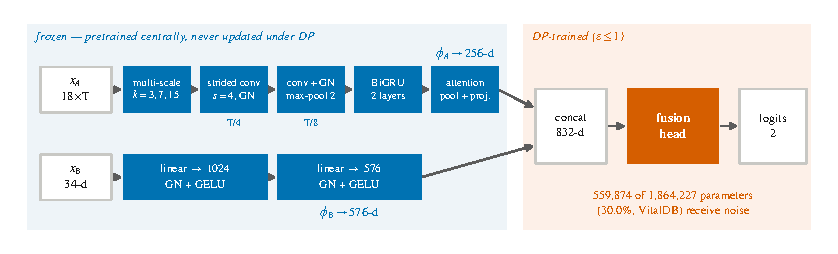
\includegraphics[width=\textwidth]{fig2_backbone.pdf}
\caption{Encoder--fusion backbone (VitalDB). Encoders are pretrained and frozen; only the fusion head ($559{,}874$ parameters) is privatized.}
\label{fig:backbone}
\end{figure*}

\subsection{Patient-Level Private Training}
\label{sec:method:privacy}
This stage ensures that each patient, and not each record, has bounded
influence on the model. The mechanism fixes the unit at the point of clipping
rather than recovering it afterwards; Fig.~\ref{fig:unit}(a) contrasts the
two. At each optimization step, client $k$
draws a Poisson sample $S \subseteq \mathcal{P}_k$, including each patient
independently with probability
\begin{equation}
q_k = \min\big(1,\ B/|\mathcal{P}_k|\big),
\label{eq:q}
\end{equation}
where $B$ is the expected number of patients per step. For each sampled
patient, the gradients of all of that patient's records are summed and the sum
is clipped,
\begin{equation}
g_p = \!\!\sum_{(x,y)\in W_p}\!\! \nabla_{\theta_{\mathrm{head}}}\,
       \ell\big(f_\theta(x), y\big), \qquad
\bar{g}_p = g_p \min\!\Big(1, \frac{C}{\lVert g_p \rVert_2}\Big).
\label{eq:clip}
\end{equation}
Because the bound is applied to the sum, patient $p$ changes the aggregate by
at most $C$ irrespective of $k_p$; clipping each record would admit $k_p C$.
Gaussian noise scaled to the same norm is added once per step, and the result
is divided by the \emph{expected} batch size,
\begin{equation}
\tilde{g} = \frac{1}{q_k |\mathcal{P}_k|}\Big( \sum_{p \in S} \bar{g}_p
+ \mathcal{N}\big(0, \sigma_k^2 C^2 I\big) \Big),
\label{eq:noise}
\end{equation}
after which $\theta_{\mathrm{head}} \leftarrow \theta_{\mathrm{head}} - \eta
\tilde{g}$; the implementation passes $\tilde{g}$ to Adam instead, which acts
only on the released gradient and is post-processing. The divisor must not be the realized $|S|$: the noise norm reveals
the divisor, $|S|$ depends on whether a given patient is present, and
normalizing by it releases information the accountant does not cover. For the
same reason a step whose sample is empty still releases the noise.
Algorithm~\ref{alg:patientdp} states the procedure. For compute, at most
$64$ records of a patient enter $g_p$; the rule is fixed and public, so the
guarantee is unaffected, and it truncates $4.1\,\%$ of eICU patients
($3.5\,\%$ of training windows) and no VitalDB patient.

\emph{Objective solved.} Without clipping, the expected step is
$\mathbb{E}[\tilde{g}] = |\mathcal{P}_k|^{-1}\sum_{p}g_p
= \bar{k}_k\,\nabla F_k(\theta)$, where $F_k$ is the record mean of
\eqref{eq:objective} on client $k$ and $\bar{k}_k = n_k/|\mathcal{P}_k|$.
A local pass takes $|\mathcal{P}_k|/B$ such steps, $\bar{k}_k$ times fewer
than a record-level pass with $B$ records per step, so to first order in
$\eta$ both displace client $k$ by $\eta\,(n_k/B)\,\nabla F_k$: before
clipping the patient-level mechanism targets \eqref{eq:objective} with
unchanged client weights, in fewer and larger steps. The argument is for the
plain gradient step; Adam rescales coordinates adaptively, so in the
implementation it holds only approximately. Clipping is what changes
the objective: each patient's summed gradient is bounded as a whole, the
surrogate of user-level DP-SGD \cite{ref11}, which down-weights patients
whose summed gradient exceeds $C$, typically those with many records. This
change belongs to the unit and is part of its measured cost
(Section~\ref{sec:results:k}).

\begin{figure}[!t]
\centering
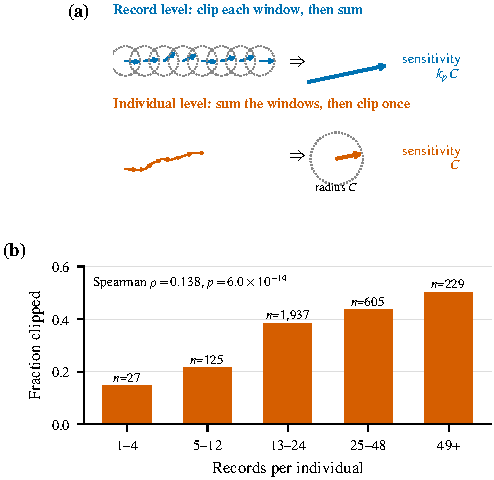
\includegraphics[width=\columnwidth]{fig02_privacy_unit.pdf}
\caption{Unit of the guarantee. (a) Per-window versus per-patient clipping. (b) Fraction of eICU individuals clipped at $C = 1$ against records contributed.}
\label{fig:unit}
\end{figure}

\begin{algorithm}[!t]
\caption{Patient-level private local update at client $k$}
\label{alg:patientdp}
\begin{algorithmic}[1]
\REQUIRE frozen $\theta_{\mathrm{enc}}$; head $\theta_{\mathrm{head}}$;
         patients $\mathcal{P}_k$ with records $\{W_p\}$; clip $C$;
         multiplier $\sigma_k$ from \eqref{eq:sigma}; rate $q_k$ from
         \eqref{eq:q}; step size $\eta$
\FOR{each local step}
  \STATE Sample $S \subseteq \mathcal{P}_k$, each $p$ independently w.p. $q_k$
  \FOR{$p \in S$}
    \STATE $g_p \leftarrow \sum_{(x,y)\in W_p}
            \nabla_{\theta_{\mathrm{head}}} \ell(f_\theta(x),y)$
            \hfill $\triangleright$ group by patient
    \STATE $\bar g_p \leftarrow g_p \cdot \min(1, C/\lVert g_p\rVert_2)$
            \hfill $\triangleright$ bound the sum
  \ENDFOR
  \STATE $\tilde g \leftarrow \big(\sum_{p\in S}\bar g_p
          + \mathcal{N}(0,\sigma_k^2C^2I)\big)/(q_k|\mathcal{P}_k|)$
          \hfill $\triangleright$ also if $S=\emptyset$
  \STATE $\theta_{\mathrm{head}} \leftarrow \theta_{\mathrm{head}} - \eta\,\tilde g$
\ENDFOR
\RETURN $\theta_{\mathrm{head}}$
\end{algorithmic}
\end{algorithm}

\subsection{Per-Client Noise Calibration}
\label{sec:method:calib}
This stage sets how much noise each client adds. Clients partitioned by
institution differ greatly in size, and therefore in
sampling rate: a small client samples a large fraction of its patients per
step. A single multiplier calibrated for the most demanding client satisfies
the budget everywhere but imposes that client's noise on all others; on eICU,
a hospital of fifteen patients sampled at $q_k = 1$ would set the noise of all
$187$ clients. When each patient is held by exactly one client (A1), the
clients' mechanisms act on disjoint individuals, and by parallel composition a
patient's guarantee is that of the client holding them; individuals held by
several clients are treated in the scope statement of Section~\ref{sec:method:privacy}. Each client therefore
uses the smallest multiplier that meets the training budget for its own
sampling rate and step count,
\begin{equation}
\begin{aligned}
\sigma_k &= \min\big\{\sigma :\ \varepsilon_k(\sigma, q_k, T_k) \le \varepsilon\big\},\\
T_k &= R\,\tau_e \max\big(1, \lfloor |\mathcal{P}_k|/B \rfloor\big),
\end{aligned}
\label{eq:sigma}
\end{equation}
where $\varepsilon_k$ is computed by the privacy loss distribution accountant
\cite{ref33}, a tight upper bound for the subsampled Gaussian mechanism, and
$T_k$ must equal the number of steps the client actually executes. Since
$\sigma_k$ depends only on the declared, public $|\mathcal{P}_k|$ and $T_k$,
using a different multiplier per client releases nothing further. Arm-versus-arm
comparisons in Section~\ref{sec:results} use the single conservative
multiplier $\sigma^{\star} = \max_k \sigma_k$ with R\'enyi accounting
\cite{ref7, ref29}, which holds every arm to the same noise.

\subsection{Hierarchical Aggregation and Update Encoding}
\label{sec:method:agg}
This stage combines the clients' private updates while keeping the uplink
small. Within a cloud round $r$, each client initializes from its edge model,
performs one private local pass, and transmits its encoded update. Edge $e$
and the cloud compute
\begin{equation}
\theta_e^{(r,s)} = \!\!\sum_{k:e(k)=e}\!\!\frac{n_k}{N_e}\,\theta_k^{(r,s)},
\qquad
\theta^{(r)} = \sum_{e=1}^{E}\frac{N_e}{n}\,\theta_e^{(r,\tau_e)},
\label{eq:agg}
\end{equation}
with $N_e = \sum_{k:e(k)=e} n_k$ (Algorithm~\ref{alg:round}). The weights
are public constants; weights
computed from the records drawn in a round would depend on which patients were
sampled and would leave the client unprotected. With $\tau_e = 1$ the edge
tier collapses into conventional single-tier federated averaging. Each update
$\Delta$ of dimension $d$ is sparsified to its $\kappa d$ largest-magnitude
coordinates and the retained values are uniformly quantized to $b$ bits,
\begin{equation}
Q(v) = v_{\min} + \operatorname{round}\!\Big(\frac{v - v_{\min}}{s}\Big)\, s,
\qquad s = \frac{v_{\max}-v_{\min}}{2^{b}-1},
\label{eq:quant}
\end{equation}
with the suppressed residual accumulated locally and added to the next
update. Both operations act on the already-perturbed head and are
post-processing.

\begin{algorithm}[!t]
\caption{PP-HFM cloud round $r$}
\label{alg:round}
\begin{algorithmic}[1]
\REQUIRE global model $\theta^{(r-1)}$; edge map $e(\cdot)$; edge rounds $\tau_e$
\STATE $\theta_e^{(r,0)} \leftarrow \theta^{(r-1)}$ for every edge $e$
\FOR{$s = 1$ \TO $\tau_e$}
  \FOR{each client $k$ \textbf{in parallel}}
    \STATE $\theta_k^{(r,s)} \leftarrow$ Algorithm~\ref{alg:patientdp}
           from $\theta_{e(k)}^{(r,s-1)}$
    \STATE transmit $Q\big(\text{top-}\kappa(\theta_k^{(r,s)}-\theta_{e(k)}^{(r,s-1)})\big)$
  \ENDFOR
  \STATE each edge aggregates by \eqref{eq:agg} (left)
\ENDFOR
\STATE cloud aggregates by \eqref{eq:agg} (right) and broadcasts $\theta^{(r)}$
\RETURN $\theta^{(r)}$
\end{algorithmic}
\end{algorithm}

\subsection{Privacy Analysis}
\label{sec:method:analysis}
This subsection proves that, under three conditions, the procedure above
protects every training patient, states what the protection costs, and lists every quantity the
system releases. Three conditions are assumed. (A1) Each patient's records lie in the training
split of exactly one client, and the training cohort is disjoint in patients
from the validation cohort, which serves checkpoint selection. (A2) The architecture, the encoder
parameters, which are pretrained on a patient-disjoint pool, all
hyperparameters, the edge map, the standardization constants and the
declared client sizes $|\mathcal{P}_k|$ and $n_k$ are public and fixed before
training; $q_k$, $T_k$, $\sigma_k$ and the weights of \eqref{eq:agg} are
computed from them and never from the data. (A3) The forward pass of a record depends on that record
alone.

\begin{theorem}[Patient-level guarantee]
\label{thm:guarantee}
Under (A1)--(A3), let each $\sigma_k$ satisfy \eqref{eq:sigma}. The transcript
of a PP-HFM run, consisting of every encoded client update, every edge and
cloud model and the model selected on the validation cohort, is
$(\varepsilon,\delta)$-differentially private with respect to each
training patient, under adding or removing all records of one patient with
the parameters of (A2) held fixed.
\end{theorem}

\begin{IEEEproof}
Fix a training patient $p$, held by client $k$ by (A1). \emph{One step.} Given
the model entering a step, the clipped gradients $\bar g_{p'}$, $p' \neq p$,
are unaffected by $p$ by (A3), and $\lVert \bar g_p\rVert_2 \le C$ by
\eqref{eq:clip}. The noisy sum in \eqref{eq:noise} is therefore a
Poisson-subsampled Gaussian mechanism with rate $q_k$, noise $\sigma_k C$ and
$\ell_2$-sensitivity $C$, whose privacy loss is bounded in
\cite{ref29, ref33}; division by the public constant $q_k|\mathcal{P}_k|$ and
the update are post-processing. \emph{Composition.} Each step takes as input
earlier outputs, other clients' messages and public quantities, so the $T_k$
steps compose adaptively, and \eqref{eq:sigma} ensures $\varepsilon_k \le \varepsilon$ at $\delta$. \emph{Other clients.} By (A1) no
other client accesses the records of $p$; its outputs are randomized
functions of its own data and of already-released messages and contribute no
privacy loss with respect to $p$. Since $\sigma_{k'}$ depends only on public
quantities, the per-client multipliers release nothing. \emph{Hierarchy.}
Sparsification with a local residual, quantization, averaging with the public
weights of \eqref{eq:agg} and broadcast are functions of released outputs and
public quantities, and selection on the validation cohort uses data disjoint
from $p$; all are post-processing.
\end{IEEEproof}

\emph{Adjacency and public sizes.} Adding or removing a patient changes the
realized cohort, but not the mechanism: the rate, step count, multiplier,
divisor and aggregation weights are fixed by the declared sizes before
training, so both neighbouring datasets are processed by the same mechanism.
This is the setting in which the Poisson-subsampled Gaussian is analyzed
\cite{ref29, ref33}; it needs no knowledge of the realized dataset and its
guarantee holds for a dataset of any size. The declared sizes are themselves
released. In the experiments they equal the realized cohort sizes, which
institutions typically publish; where a size is sensitive, it can be replaced
by a coarse public value or released by a private count at a small additional
budget, and the theorem holds for whichever declared values are used. \emph{Standardization.} The theorem holds with the standardization
constants fixed, like the declared sizes; with the constants recomputed after
a patient is removed, every other record would be represented differently.
In the experiments the constants are fitted once on the training cohort, so
their release is outside the guarantee (Table~\ref{tab:ledger}). Its size was
measured on eICU, where the fit can be reproduced exactly: removing one
individual moves any mean by at most $0.0017$ standard deviations and, for
$99\,\%$ of individuals, any standard deviation by at most $0.02\,\%$, but
the most extreme outlier moves one channel's standard deviation by
$5.2\,\%$. Constants fitted on the disjoint pretraining pool alone differ
from those used by at most $0.026$ standard deviations in mean and
$4.4\,\%$ in scale. On eICU the headline is therefore repeated with
constants fitted on the disjoint pool and encoders pretrained in those units
(Section~\ref{sec:results:privacy}); there every input to the private head is
either public or covered by the theorem.

Table~\ref{tab:ledger} lists every release of the headline configuration;
the unit comparison and the audit use $\varepsilon = 1.0 + 0.5$ with one
worst-client multiplier (Table~\ref{tab:scope}). The protected population is
the training cohort; validation patients select the checkpoint without noise
and are outside the guarantee, as is conventional \cite{ref6}.

\begin{table}[!t]
\centering
\caption{Privacy ledger of the headline configuration: every release and the
population it touches. Table~\ref{tab:scope} gives the other configurations.}
\label{tab:ledger}
\setlength{\tabcolsep}{2.4pt}
\footnotesize
\begin{tabular}{lll}
\toprule
Release & Population & Protection \\
\midrule
Client updates, edge/cloud models & training & $(0.9, 10^{-5})$-DP per client \\
Selected checkpoint               & validation & none \\
Conformal threshold (evaluated)   & validation & $\varepsilon_{\mathrm{conf}} = 0.1$ \\
Standardization (headline runs) & training & none \\
Standardization (eICU rerun) & public pool & public \\
Declared sizes, $q_k$, $T_k$, $\sigma_k$ & -- & public by design \\
Encoders (disjoint pool)          & external & not required \\
Encoders (oracle)                 & training & violates (A2) \\
\bottomrule
\end{tabular}
\end{table}

% Table IV (scope) is defined here, beside Table III, so the full-width float
% reaches the top of the page that explains it (it lands one page after definition).
\begin{table*}[!t]
\centering
\caption{Scope of the guarantee in each evaluated configuration}
\label{tab:scope}
\footnotesize
\setlength{\tabcolsep}{4pt}
\begin{tabular}{>{\raggedright\arraybackslash}p{4.8cm}>{\raggedright\arraybackslash}p{2.3cm}>{\raggedright\arraybackslash}p{3.6cm}>{\raggedright\arraybackslash}p{3.3cm}>{\raggedright\arraybackslash}p{2.7cm}}
\toprule
Configuration & Unit & Encoders / standardization & Accounting & Guarantee covers \\
\midrule
eICU, headline (one hospital per person) & patient & disjoint / training cohort & $\sigma_k$, PLD; $0.9 + 0.1$ & training transcript \\
eICU, pool-fitted constants (one hospital per person) & patient & disjoint / public pool & $\sigma_k$, PLD; $0.9 + 0.1$ & end to end \\
VitalDB, person-level headline & person & oracle / training cohort & $\sigma_k$, PLD; $0.9 + 0.1$ & transcript; (A2) violated \\
VitalDB, disjoint encoders (case-level) & surgical case & disjoint / training cohort & $\sigma_k$, PLD; $0.9 + 0.1$ & transcript, per case \\
VitalDB, cost of the unit and audit (person-level) & person vs record & oracle / training cohort & $\sigma_{\max}$, RDP; $1.0 + 0.5$ & training transcript \\
Scaling grids, clipping rule (VitalDB case-level; eICU) & individual vs record & oracle (VitalDB), disjoint (eICU) / training & $\sigma_{\max}$, RDP; $0.8$--$1.0 + 0.2$--$0.5$ & training transcript$^{\ddagger}$ \\
eICU, prior systems (source partition) & patient & disjoint / training cohort & $\sigma_k$, PLD; $0.9 + 0.1$ & training transcript$^{\ddagger}$ \\
WEAR & record (= participant) & oracle / training cohort & record-level; $0.766 + 0.2$ & transcript, per record \\
\bottomrule
\end{tabular}
\tabnote{Unit: neighboring datasets differ by all records of one patient, person or case, or by one record; ``vs'' marks a comparison of two arms. Accounting: $\varepsilon_{\mathrm{train}} + \varepsilon_{\mathrm{conf}}$ at $\delta = 10^{-5}$; $\sigma_k$, per-client multipliers; $\sigma_{\max}$, one worst-client multiplier; PLD, privacy-loss-distribution accountant; RDP, R\'enyi accountant. The conformal release was evaluated and is not part of the deployed system. Arms compared with each other share one configuration. Other analyses (recipe, ablation, fusion, attribution) are labeled with their partition and mechanism in Section~\ref{sec:results}. $^{\ddagger}$eICU on the source partition: for the $97.1\,\%$ of training persons at one hospital; the $2.9\,\%$ at two to four hospitals compose the mechanisms of those hospitals ($\varepsilon_{\mathrm{train}} \le 1.32$--$1.92$ with $\sigma_k$ and PLD).}
\end{table*}

\begin{corollary}[Coincidence of the units]
\label{cor:k1}
If every patient contributes one record, Algorithm~\ref{alg:patientdp} is
DP-SGD with Poisson sampling over records. For equal $(B, T_k, \sigma, C)$,
the patient- and record-level mechanisms are then the same mechanism, so any
difference between them at one record per patient measures seed variation or
an implementation difference, not the privacy unit.
\end{corollary}

The theorem bounds what the guarantee reveals; the next statement predicts
what it costs. Suppose $P$ individuals each contribute exactly $k$ records.
The record-level arm minimizes $\frac{1}{Pk}\sum_p\sum_{w\in W_p}\ell_w$, and
the patient-level arm minimizes the same objective written as
$\frac{1}{P}\sum_p \bar\ell_p$ with $\bar\ell_p = \frac{1}{k}\sum_{w\in
W_p}\ell_w$.

\begin{proposition}[Cost in records per individual]
\label{prop:scaling}
Let each $\ell_w$ be convex and $L$-Lipschitz on a domain of diameter $D$ in
$\mathbb{R}^d$, and let both arms be trained by private gradient descent at
the same $(\varepsilon,\delta)$, and let $\Lambda =
LD\sqrt{d\log(1/\delta)}/\varepsilon$. (i) The excess empirical risk of the
record-level arm is at most $c_{\mathrm{rec}}\Lambda/(Pk)$ and that of the
patient-level arm at most $c_{\mathrm{ind}}\Lambda/P$, with constants
independent of $k$; both rates are tight in the worst case up to logarithmic factors. (ii) If both arms
attain their rate with a common constant $c$, the gap is $A(1 - 1/k)$ with
$A = c\Lambda/P$.
\end{proposition}

\begin{IEEEproof}
For $n$ units with convex $L$-Lipschitz losses, private gradient descent
attains excess risk $O(LD\sqrt{d\log(1/\delta)}/(n\varepsilon))$, and the rate
is tight up to logarithmic factors \cite{ref31}. The record-level arm has $n = Pk$ units. In the
patient-level arm the unit is $\bar\ell_p$, which is $L$-Lipschitz as an
average of $L$-Lipschitz losses; clipping the summed gradient at $C$ equals
clipping the gradient of $\bar\ell_p$ at $C/k$, a rescaling that leaves the
guarantee unchanged, so the mechanism is private gradient descent over $n = P$
units. This gives (i), and (ii) follows by subtraction.
\end{IEEEproof}

Part (ii) rests on an assumption that (i) does not supply: upper bounds with
different constants do not determine the attained gap. The form
$A(1-1/k)$ is therefore a \emph{scaling hypothesis} that the proposition
motivates, not a theorem, and it is tested empirically, including out of
sample. Since the head is not convex and the reported metric is not excess
risk, the hypothesis concerns the \emph{shape} of the cost, not its
magnitude: one free parameter, zero at $k = 1$, and a patient-level arm whose
utility does not depend on $k$. It also indicates what would recover
the cost: mechanisms that clip around an estimate of each individual's mean
gradient attain user-level rates that improve with $k$ \cite{ref32}, whereas
a bound fixed around zero cannot.

\emph{Scope.} On eICU and on the person-level VitalDB partition the unit is
the person. On the case-level VitalDB partition it is the surgical case:
$230$ of $5{,}974$ people ($3.9\,\%$) underwent more than one operation, and
for them the guarantee extends to the person only by group privacy over at
most $14$ cases, composed across clients for the $68$ training persons whose
cases lie on two. On eICU, where clients are hospitals, the stays of $2{,}177$ of $74{,}327$ training persons ($2.9\,\%$) lie at two to four hospitals, so in the source partition (A1) fails for them. The privacy-cost and end-to-end runs therefore use a partition in which each such person is moved, with all their records, to the hospital holding most of their stays ($49{,}939$ training records; likewise $509$ validation and $589$ test persons); no record is excluded and every split is unchanged. In that partition every training and validation person is held by one hospital, so (A1) holds and the guarantee is $\varepsilon_{\mathrm{train}} = 0.9$ for every training person, verified independently for every client of every run (privacy-loss-distribution bounds $[0.880, 0.900]$; R\'enyi accountant $0.974$), and the evaluated conformal release adds $\varepsilon_{\mathrm{conf}} = 0.1$ once per person. The remaining eICU analyses (system objectives other than O2, scaling grid, clipping rule and prior systems) use the source partition, in which the per-client budget composes across the hospitals that hold a person: with the headline accountant, at most $1.32$, $1.64$ and $1.92$ for the $2{,}097$, $75$ and $5$ persons at two, three and four hospitals (R\'enyi: $1.42$, $1.77$, $2.08$), and at most $m\varepsilon$ in general; arms compared with each other share the partition. On WEAR each client is one participant, client-, user- and
record-level units coincide at the client, and the mechanism evaluated there
is record-level. The guarantee holds end to end only with the disjoint
encoders and pool-fitted standardization constants; the oracle encoders
violate (A2), and training-fitted constants are an unprotected release. Table~\ref{tab:scope} lists, for each evaluated configuration, the unit,
the provenance of the encoders and standardization constants, the accounting
and what the guarantee covers. The implementation of the accounting is
additionally checked by a suite of 17 regression checks, seven of which cover
it: composition of the budget across calls, release and accounting of noise at
every step with the expected-batch divisor, one conformal score per calibration
patient, and per-client multipliers within the budget. These are
implementation-level checks of the accounting configuration; they do not by
themselves establish the guarantee.


\subsection{Empirical Audit}
\label{sec:method:mia}
A proof bounds what an adversary can learn; an audit measures what a concrete
attack actually achieves. The guarantee is audited by patient-level membership inference. Members are
training patients and non-members are held-out patients, scored by the same
released model. Two attacks are used: thresholding of a patient's mean loss
\cite{ref15}, and LiRA \cite{ref17} adapted to the patient unit. Sixteen
shadow models are trained on independently drawn halves of the patient
population, with all records of a patient assigned together. For each patient,
the logit-scaled confidence averaged over their records,
\begin{equation}
\varphi(p) = \frac{1}{k_p}\sum_{(x,y)\in W_p}
\Big( z_y(x) - \log\!\sum_{j \neq y} e^{z_j(x)} \Big),
\label{eq:phi}
\end{equation}
is modeled by Gaussians fitted over the shadows that include and exclude the
patient (Fig.~\ref{fig:lira}), and membership is scored by
$\Lambda(p) = \log \mathcal{N}(\varphi;\mu_{\mathrm{in}},\sigma^2_{\mathrm{in}})
- \log \mathcal{N}(\varphi;\mu_{\mathrm{out}},\sigma^2_{\mathrm{out}})$.
A negative result is accepted only if the same procedure detects clearly
elevated leakage on a positive control, non-private training of the same head
over the same encoders. Attack AUCs are compared with a difficulty floor,
the AUC obtained by ranking patients by their mean statistic over the shadows
that exclude them, without the target model, because members and non-members
may differ in intrinsic difficulty. The audited models are the five-seed
record- and patient-level models of the unit comparison
(Section~\ref{sec:results:privacy}), trained at $\varepsilon = 1$, a slightly
weaker budget than the headline, so the audit is conservative.

\begin{figure}[!t]
\centering
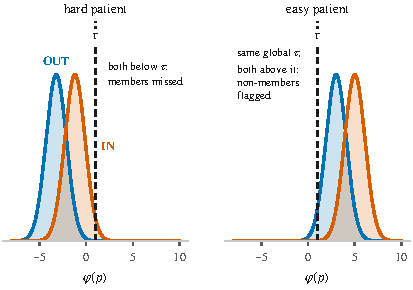
\includegraphics[width=\columnwidth]{fig4_lira.pdf}
\caption{Per-patient calibration in LiRA (illustrative): a global threshold misclassifies hard and easy patients that per-patient IN/OUT fits separate.}
\label{fig:lira}
\end{figure}

\subsection{Deployment and Instrumentation}
The trained network is exported to a portable graph and executed at full
precision on a CPU provider at the edge, so the wide-area link is not on the
inference path. Latency is decomposed into preprocessing, forward pass
and post-processing, and is reported at the
$95$th percentile over $1{,}000$ timed runs after $100$ warm-up runs.
Communication delay, delivery and traffic are measured in a packet-level
network simulation of the three tiers, with a wireless local-area
device-to-edge link and a point-to-point backhaul, on every simulated round.
Energy is modeled per tier, because a hierarchy redistributes work, and an
aggregate figure would hide a saving at one tier offset by a cost at another.
